In diesem Abschnitt machen wir uns die getroffenen \nameref{ch:Content2:sec:a Posteriori} Annahmen 
zu Nutze. Nach dem Erzeugen von $Bild_{t}$ (und vor dem Erzeugen von $Bild_{t+1}$) nehmen wir die Sortierung
anhand der Pixelwerte von $Bild_{t}$ vor. 

\par

Die Pixel innerhalb eines Blocks (z.B. Blockgröße = 64, Auswirkung von verschiedenen Blockgrößen in Abbildung \ref{fig:VerschiedeneBlockgrößenSorting}) werden anhand ihrer 
Intensität in einer aufsteigenden Liste sortiert und damit zu einem Histogramm. Dieses generierte Histogramm wird für jeden Pixel innerhalb des Blocks verwendet.
Die sortierte Liste als Histogramm zu benutzen ist zulässig. Denn beim Benutzen der inversen Funktion \ref{eq:inverse Funktion} machen wir nichts Anderes als 
zufällige Zahlen auf ein bestimmtes Wahrscheinlichkeitsquantil, das einer gewissen Sortierung entspricht, abzubilden. Deshalb können wir die Pixelintensitäten 
innerhalb eines Blocks anhand ihrer Indizes (entspricht den Wahrscheinlichkeitsquantilen bei der Wahrscheinlichkeitsfunktion) sortieren! 

\begin{tcolorbox}
\begin{algorithm}[H]
    \caption{\textbf{Sortier Schritt t}}
    \begin{algorithmic}[1]
        \State pixel \textbf{consists of} value,index;
        \State List framePixelsIntensities, noiseIntensities;
        \State $assert(sizeof(framePixelsIntensities)==BLOCKSIZE)$;
        \State $assert(sizeof(noiseIntensities)==BLOCKSIZE)$;
        \State List L $\leftarrow$ pixels of frame t in block;
        \State \hfill
        \State //sort the two lists by means of intensities
        \State sort\_by\_means\_of\_value(framePixelsIntensities);
        \State sort\_by\_means\_of\_value(noiseIntensities);
        \State \hfill
        \State //correspondig indices are also sorted by means of values
        \For{$i = 1 .. BLOCKSIZE$}
        \State $sortedSeeds(noiseIntensities.getIndex(i)) = $
        \State $incomingSeeds(framePixelIntensities.getIndex(i))$;
        \EndFor
        \State //now the seeds are sorted following a blue noise distribution
    \end{algorithmic}
    \label{alg:Sortier}
\end{algorithm}
\end{tcolorbox}

Das Verwenden der anhand Pixel- und blue noise Werten sortierten Indizes in Zeile 13,14 des Algorithmus \ref{alg:Sortier} ist die praktische Anwendung der zuvor eingeführten 
Quantilfunktion \ref{eq:inverse Funktion}. Denn die Anfangswerte $x \in [0,1]$ der Quantilfunktion \ref{eq:inverse Funktion} werden hier einem eindeutigen sortierten Intensitätswert 
zugeteilt. Das Abbilden der Pixelwerte auf Werte einer \nameref{ch:Content1:sec:blue noise} Textur garantiert nun die entsprechende Korrelation 
der Anfangswerte zueinander (siehe auch Abschnitt \ref{ch:Content1:sec:blue noise sampling}).
Die Annahme der Lokalität, also der Homogenität (in der Abbildung \ref{fig:Pixelblöcke} demonstriert) einer Fläche innerhalb eines Blocks, 
erlaubt die Approximation des Histogramms \ref{fig:Pixelwerte} eines Pixels anhand der Intensitäten aller anderen Pixel innerhalb des Blocks.
Wird der Block zu groß gewählt, so wird die Approximation zu rechenintensiv, die parallele Ausführbarkeit 
und die  Homogenitätseigenschaft (Bildkohärenz) gehen verloren, wohingegen zu kleine Blockgrößen nur eine sehr vage und ungenaue Approximation des 
Histogramms \ref{pic:histogramOfEstimates} liefern.

\par

Hierbei muss noch eine wichtige Anmerkung gemacht werden. Die Fehlerverteilung der Pixelwerte im Bildraum konvergiert auf diese Weise nicht perfekt zu einer 
blue noise Verteilung, denn wir wechseln in jedem Bild die verwendeten blue noise Texturen(theoretisch, praktischerweise werden wir hier eine
Textur verwenden und mit Erkenntnissen aus Abschnitt \ref{ch:Content1:sec:Quasi-Zufallsfolgen} quasi-zufällig zugreifen um einen solchen Effekt zu erreichen). 

\subsubsection{Blockgöße}
\label{subsec:Blockgröße}

Für den Sortierschritt gibt es ein Abwägung zu treffen: Hohe Blockgröße B bedeutet eine bessere Approximation 
des Histogramms (siehe Bild \ref{pic:histogramOfEstimates}). Denn man erhöht die Anzahl an Pixelschätzungen für
jeden einzelnen Pixel. Allerdings geht im Gegenzug die Raum-Zeit Kohärenz verloren. Der Algorithmus wird anfälliger 
für Szenen, die keine größeren homogenen Flächen aufweisen.

\begin{figure}[H]
    \begin{tcolorbox}[boxrule=4pt,sharp corners=downhill,title=Verschiedene Blockgrößen]
    %%%%%%%%%%%%%%%%%%%%%%%%%%%%%%%%%%%%%%%%%%%%%%%%%%%%%%%%%%%%%%%%%%%%%%%%%%%%%%%%%%%%%%%%%%%%%%%%%%%%%%
    %%%%%%%%%%%%%%%%%%%%%%%%%%%%%%% first row 
    %%%%%%%%%%%%%%%%%%%%%%%%%%%%%%%%%%%%%%%%%%%%%%%%%%%%%%%%%%%%%%%%%%%%%%%%%%%%%%%%%%%%%%%%%%%%%%%%%%%%%%
    \centering
    \begin{subfigure}[b]{0.2\linewidth}
      
\includegraphics[width=\linewidth]{content/TemporalerAlg/Bilder/Sorting/DiffDimensions/2/seed_debug_5.0_small.png}
       \caption{FT B = 2}
       \label{pic:fftB_2}
    \end{subfigure}
    \begin{subfigure}[b]{0.2\linewidth}
      
\includegraphics[width=\linewidth]{content/TemporalerAlg/Bilder/Sorting/DiffDimensions/3/seed_debug_5.0_small.png}
      \caption{FT B = 3}
      \label{pic:fftB_3}
    \end{subfigure}
    \begin{subfigure}[b]{0.2\linewidth}
      
\includegraphics[width=\linewidth]{content/TemporalerAlg/Bilder/Sorting/DiffDimensions/4/seed_debug_5.0_small.png}
      \caption{FT B = 4}
      \label{pic:fftB_4}
    \end{subfigure}
    \begin{subfigure}[b]{0.2\linewidth}
        
\includegraphics[width=\linewidth]{content/TemporalerAlg/Bilder/Sorting/DiffDimensions/5/seed_debug_5.0_small.png}
        \caption{FT B = 5}
        \label{pic:fftB_5}
    \end{subfigure}
    %%%%%%%%%%%%%%%%%%%%%%%%%%%%%%%%%%%%%%%%%%%%%%%%%%%%%%%%%%%%%%%%%%%%%%%%%%%%%%%%%%%%%%%%%%%%%%%%%%%%%%
    %%%%%%%%%%%%%%%%%%%%%%%%%%%%%%% second row
    %%%%%%%%%%%%%%%%%%%%%%%%%%%%%%%%%%%%%%%%%%%%%%%%%%%%%%%%%%%%%%%%%%%%%%%%%%%%%%%%%%%%%%%%%%%%%%%%%%%%%%
    \begin{subfigure}[b]{0.2\linewidth}
        
\includegraphics[width=\linewidth]{content/TemporalerAlg/Bilder/Sorting/DiffDimensions/2/seed_debug_5.0_small_screen.png}
         \caption{B=2}
         \label{pic:screen_B2}
    \end{subfigure}
    \begin{subfigure}[b]{0.2\linewidth}
        
\includegraphics[width=\linewidth]{content/TemporalerAlg/Bilder/Sorting/DiffDimensions/3/seed_debug_5.0_small_screen.png}
         \caption{B=3}
         \label{pic:screen_B3}
    \end{subfigure}
    \begin{subfigure}[b]{0.2\linewidth}
        
\includegraphics[width=\linewidth]{content/TemporalerAlg/Bilder/Sorting/DiffDimensions/4/seed_debug_5.0_small_screen.png}
         \caption{B=4}
         \label{pic:screen_B4}
    \end{subfigure}
    \begin{subfigure}[b]{0.2\linewidth}
        
\includegraphics[width=\linewidth]{content/TemporalerAlg/Bilder/Sorting/DiffDimensions/5/seed_debug_5.0_small_screen.png}
         \caption{B=5}
         \label{pic:screen_B5}
    \end{subfigure}
    %%%%%%%%%%%%%%%%%%%%%%%%%%%%%%%%%%%%%%%%%%%%%%%%%%%%%%%%%%%%%%%%%%%%%%%%%%%%%%%%%%%%%%%%%%%%%%%%%%%%%%
    %%%%%%%%%%%%%%%%%%%%%%%%%%%%%%% third row 
    %%%%%%%%%%%%%%%%%%%%%%%%%%%%%%%%%%%%%%%%%%%%%%%%%%%%%%%%%%%%%%%%%%%%%%%%%%%%%%%%%%%%%%%%%%%%%%%%%%%%%%
    \centering
    \begin{subfigure}[b]{0.2\linewidth}
      
\includegraphics[width=\linewidth]{content/TemporalerAlg/Bilder/Sorting/DiffDimensions/6/seed_debug_5.0_small.png}
       \caption{FT B = 6}
       \label{pic:fftB_6}
    \end{subfigure}
    \begin{subfigure}[b]{0.2\linewidth}
      
\includegraphics[width=\linewidth]{content/TemporalerAlg/Bilder/Sorting/DiffDimensions/7/seed_debug_5.0_small.png}
      \caption{FT B = 7}
      \label{pic:fftB_7}
    \end{subfigure}
    \begin{subfigure}[b]{0.2\linewidth}
      
\includegraphics[width=\linewidth]{content/TemporalerAlg/Bilder/Sorting/DiffDimensions/8/seed_debug_5.0_small.png}
      \caption{FT B = 8}
      \label{pic:fftB_8}
    \end{subfigure}
    \begin{subfigure}[b]{0.2\linewidth}
        
\includegraphics[width=\linewidth]{content/TemporalerAlg/Bilder/Sorting/DiffDimensions/10/seed_debug_5.0_small.png}
        \caption{FT B = 10}
        \label{pic:fftB_10}
    \end{subfigure}
    %%%%%%%%%%%%%%%%%%%%%%%%%%%%%%%%%%%%%%%%%%%%%%%%%%%%%%%%%%%%%%%%%%%%%%%%%%%%%%%%%%%%%%%%%%%%%%%%%%%%%%
    %%%%%%%%%%%%%%%%%%%%%%%%%%%%%%% 4th row
    %%%%%%%%%%%%%%%%%%%%%%%%%%%%%%%%%%%%%%%%%%%%%%%%%%%%%%%%%%%%%%%%%%%%%%%%%%%%%%%%%%%%%%%%%%%%%%%%%%%%%%
    \begin{subfigure}[b]{0.2\linewidth}
        
\includegraphics[width=\linewidth]{content/TemporalerAlg/Bilder/Sorting/DiffDimensions/6/seed_debug_5.0_small_screen.png}
         \caption{B=6}
         \label{pic:screen_B6}
    \end{subfigure}
    \begin{subfigure}[b]{0.2\linewidth}
        
\includegraphics[width=\linewidth]{content/TemporalerAlg/Bilder/Sorting/DiffDimensions/7/seed_debug_5.0_small_screen.png}
         \caption{B=7}
         \label{pic:screen_B7}
    \end{subfigure}
    \begin{subfigure}[b]{0.2\linewidth}
        
\includegraphics[width=\linewidth]{content/TemporalerAlg/Bilder/Sorting/DiffDimensions/8/seed_debug_5.0_small_screen.png}
         \caption{B=8}
         \label{pic:screen_B8}
    \end{subfigure}
    \begin{subfigure}[b]{0.2\linewidth}
        
\includegraphics[width=\linewidth]{content/TemporalerAlg/Bilder/Sorting/DiffDimensions/10/seed_debug_5.0_small_screen.png}
         \caption{B=10}
         \label{pic:screen_B10}
    \end{subfigure}
    \end{tcolorbox}
    \caption{Verschiedene Blockgrößen B bei selben homogenen Szenenausschnitt; nur Sortierschritt}
    \label{fig:VerschiedeneBlockgrößenSorting}
\end{figure}

Generell lässt sich aus den Untersuchungen in Abbildung \ref{fig:VerschiedeneBlockgrößenSorting} schließen,
dass eine geringe Blockgröße des Sortierschrittes ein Fehlen bzw. eine starke Abschwächung der 
\nameref{ch:Content1:sec:blue noise} Fehlerverteilung im Bildraum zur Folge hat. Erklärung: Das Histogramm
(siehe Abbildung \ref{pic:histogramOfEstimates}), Wahrscheinlichkeitsfunktion
aller möglichen Pixelwerte, wird mit zu wenigen Werten approximiert. Diese sehr vage Approximation 
hat zur Folge, dass die Sortierung einer randomisierten Folge entspricht. Deshalb sind im Bildraum
viele Cluster und die white noise Eigenschaften in den Spektra zu erkennen.
Unsere Untersuchungen ergeben, dass eine Blockgröße < 4 vermieden werden sollte. Ab einer Blockgröße
B = 4 hat man bereits eine rechengünstige benutzbare Approximation. Eine gute Abschätzung ergibt sich 
bei uns mit einer Blockgröße von $B \approx 8/10$. Mit dieser Blockgröße hat man immernoch eine gute, 
effiziente, parallele Ausführbarkeit garantiert und liefert eine generelle, gute Approximation der 
Pixelwerte.   

%%%%%%%%%%%%%%%%%%%%%%%%%%%%%%%%%%%%%%%%%%%%%%%%%%%%%%%%%%%%%%%%%%%%%%%%%%%%%%%%%%%%%%%%%%%%%%%%%%%%%%
%%%%%%%%%%%%%%%%%%%%%%%%%%%%%%% Histogramm Verdeutlichung
%%%%%%%%%%%%%%%%%%%%%%%%%%%%%%%%%%%%%%%%%%%%%%%%%%%%%%%%%%%%%%%%%%%%%%%%%%%%%%%%%%%%%%%%%%%%%%%%%%%%%%

\begin{figure}[H]
    \centering
    \begin{subfigure}{0.4\textwidth}
        \centering\includegraphics[width=\linewidth]{content/TemporalerAlg/Bilder/Sorting/Histogramm/HistogrammSchätzungPrevious.png} 
        \caption{Vorheriges Bild}
        \label{fig:Histogramm_Previous}
    \end{subfigure}
    \centering
    \begin{subfigure}{0.4\textwidth}
        \centering\includegraphics[width=\linewidth]{content/TemporalerAlg/Bilder/Sorting/Histogramm/HistogrammSchätzungPostBearbeitet.png}
        \caption{Nach Verschiebung}
        \label{fig:Histogram_Post}
    \end{subfigure}
    \caption{Wir sortieren unsere Anfangswerte und erhalten durch die Pixelwertschätzungen in der Umgebung eine gute Approximation im ersten Bild
    \ref{fig:Histogramm_Previous}; Verschieben wir die Anfangswertetextur ohne weiter zu sortieren, so werden nun Anfangswerte, die anhand der Pixelwertschätzung des
    Posters verwendet wurden, nun zur Pixelfarbgebung für die Wand verwendet (grünes Rechteck). Mann kann sehen, dass hier keine blue noise Eigenschaft mehr zu erkennen
    ist, da die Pixelwertschätzungen des Posters nicht auf die Wand übertragbar sind! Hingegen kann man im blauen Rechteck eine blue noise Eigenschaft erkennen, da 
    die verwendeten Anfangswerte anhand einer ähnlich farbigen Oberfläche sortiert wurden.} 
    \label{fig:Vergleich der Histogramme}
\end{figure}

%%%%%%%%%%%%%%%%%%%%%%%%%%%%%%%%%%%%%%%%%%%%%%%%%%%%%%%%%%%%%%%%%%%%%%%%%%%%%%%%%%%%%%%%%%%%%%%%%%%%%%
%%%%%%%%%%%%%%%%%%%%%%%%%%%%%%% Screenshotreihe
%%%%%%%%%%%%%%%%%%%%%%%%%%%%%%%%%%%%%%%%%%%%%%%%%%%%%%%%%%%%%%%%%%%%%%%%%%%%%%%%%%%%%%%%%%%%%%%%%%%%%%

\newpage

%%%%%%%%%%%%%%%%%%%%%%%%%%%%%%%%%%%%%%%%%%%%%%%%%%%%%%%%%%%%%%%%%%%%%%%%%%%%%%%%%%%%%%%%%%%%%%%%%%%%%%
%%%%%%%%%%%%%%%%%%%%%%%%%%%%%%% first row; starting point scene
%%%%%%%%%%%%%%%%%%%%%%%%%%%%%%%%%%%%%%%%%%%%%%%%%%%%%%%%%%%%%%%%%%%%%%%%%%%%%%%%%%%%%%%%%%%%%%%%%%%%%%  
\begin{figure}[H]
        \centering 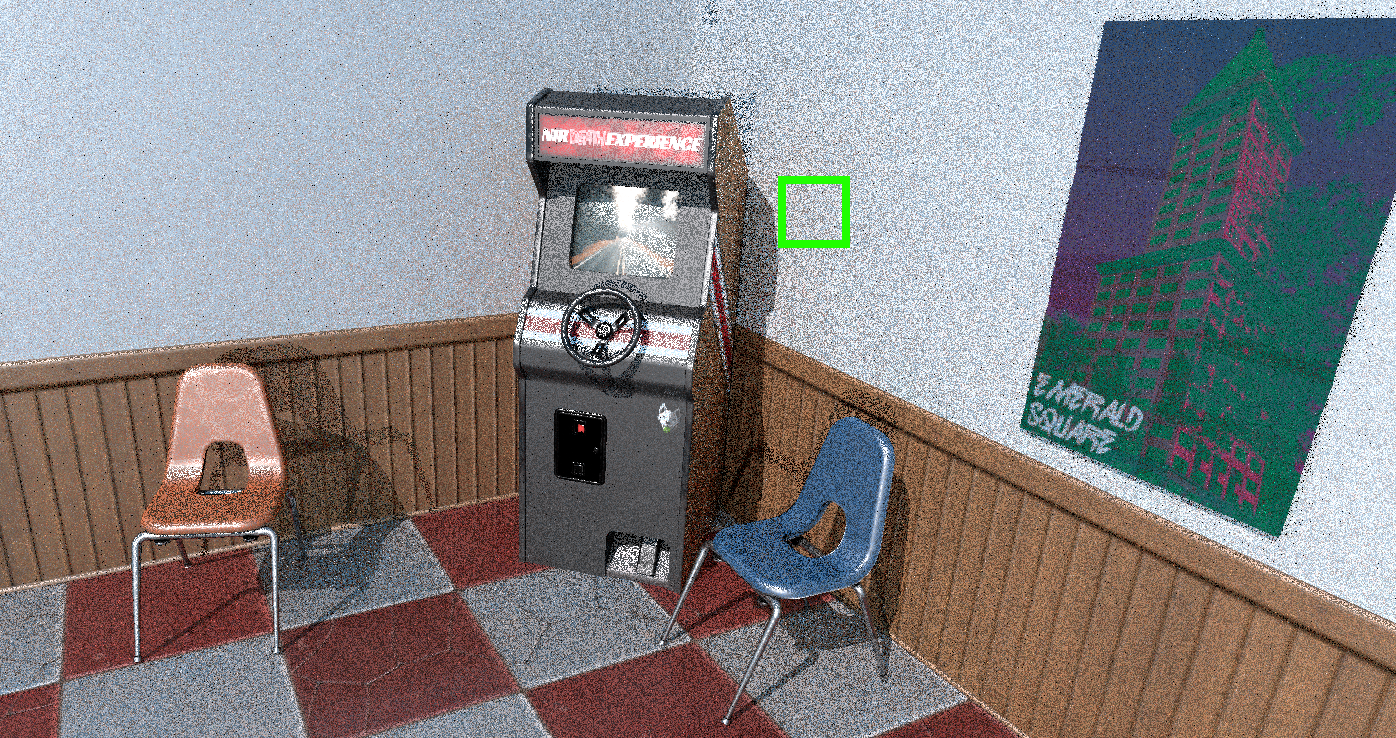
\includegraphics[scale=.25]{content/TemporalerAlg/Bilder/Sorting/Szene/Szene1.png}
        \caption{Szene vor eingeschalteten Sortieren, Ausschnitt(grüner Kasten wird über mehrere 
        Bilder nach Aktivierung des Sortierens verfolgt)}
        \label{fig:Nur_Sorting_Szene_t1}
\end{figure}

%%%%%%%%%%%%%%%%%%%%%%%%%%%%%%%%%%%%%%%%%%%%%%%%%%%%%%%%%%%%%%%%%%%%%%%%%%%%%%%%%%%%%%%%%%%%%%%%%%%%%%
%%%%%%%%%%%%%%%%%%%%%%%%%%%%%%% second row; ausschnitt over time
%%%%%%%%%%%%%%%%%%%%%%%%%%%%%%%%%%%%%%%%%%%%%%%%%%%%%%%%%%%%%%%%%%%%%%%%%%%%%%%%%%%%%%%%%%%%%%%%%%%%%%  
\begin{figure}[H]
    \begin{tcolorbox}[boxrule=4pt,sharp corners=downhill,title=Sortieren]
    %%%%%%%%%%%%%%%%%%%%%%%%%%%%%%%%%%%%%%%%%%%%%%%%%%%%%%%%%%%%%%%%%%%%%%%%%%%%%%%%%%%%%%%%%%%%%%%%%%%%%%
    %%%%%%%%%%%%%%%%%%%%%%%%%%%%%%% first ausschnitt row
    %%%%%%%%%%%%%%%%%%%%%%%%%%%%%%%%%%%%%%%%%%%%%%%%%%%%%%%%%%%%%%%%%%%%%%%%%%%%%%%%%%%%%%%%%%%%%%%%%%%%%%  
    \begin{subfigure}[b]{0.2\textwidth}
        \centering
        
\includegraphics[width=\textwidth]{content/TemporalerAlg/Bilder/Sorting/Ausschnitte/Ausschnitt1.png}
        \caption{t=1}
        \label{pic:sorting_t1}
    \end{subfigure}
    \begin{subfigure}[b]{0.2\textwidth}
        \centering
        
\includegraphics[width=\textwidth]{content/TemporalerAlg/Bilder/Sorting/Spektren/Ausschnitt1.png}
        \subcaption{FFT t=1}
        \label{pic:sorting_t1_FFT}
    \end{subfigure}
    \begin{subfigure}[b]{0.1\textwidth}
        \hspace*{1cm}
    \end{subfigure}
    \begin{subfigure}[b]{0.2\textwidth}
        \centering
        
\includegraphics[width=\textwidth]{content/TemporalerAlg/Bilder/Sorting/Ausschnitte/Ausschnitt5.png}
        \subcaption{FFT t=5}
        \label{pic:sorting_t5}
    \end{subfigure}
    \begin{subfigure}[b]{0.2\textwidth}
        \centering
        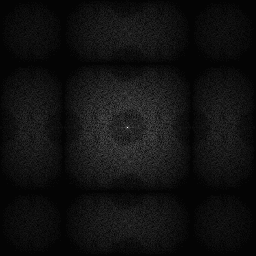
\includegraphics[width=\textwidth]{content/TemporalerAlg/Bilder/Sorting/Spektren/Ausschnitt5.png}
        \subcaption{FFT t=5}
        \label{pic:sorting_t5_FFT}
    \end{subfigure}
    %%%%%%%%%%%%%%%%%%%%%%%%%%%%%%%%%%%%%%%%%%%%%%%%%%%%%%%%%%%%%%%%%%%%%%%%%%%%%%%%%%%%%%%%%%%%%%%%%%%%%%
    %%%%%%%%%%%%%%%%%%%%%%%%%%%%%%% second row; ausschnitt over time
    %%%%%%%%%%%%%%%%%%%%%%%%%%%%%%%%%%%%%%%%%%%%%%%%%%%%%%%%%%%%%%%%%%%%%%%%%%%%%%%%%%%%%%%%%%%%%%%%%%%%%%  
    \begin{subfigure}[b]{0.2\textwidth}
        \centering
        
\includegraphics[width=\textwidth]{content/TemporalerAlg/Bilder/Sorting/Ausschnitte/Ausschnitt2.png}
        \caption{t=2}
        \label{pic:sorting_t2}
    \end{subfigure}
    \begin{subfigure}[b]{0.2\textwidth}
        \centering
        
\includegraphics[width=\textwidth]{content/TemporalerAlg/Bilder/Sorting/Spektren/Ausschnitt2.png}
        \subcaption{FFT t=2}
        \label{pic:sorting_t2_FFT}
    \end{subfigure}
    \begin{subfigure}[b]{0.1\textwidth}
        \hspace*{1cm}
    \end{subfigure}
    \begin{subfigure}[b]{0.2\textwidth}
        \centering
        
\includegraphics[width=\textwidth]{content/TemporalerAlg/Bilder/Sorting/Ausschnitte/Ausschnitt6.png}
        \subcaption{FFT t=6}
        \label{pic:sorting_t6}
    \end{subfigure}
    \begin{subfigure}[b]{0.2\textwidth}
        \centering
        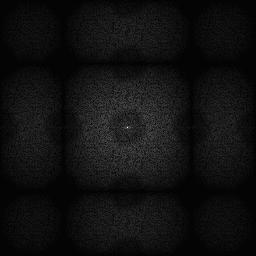
\includegraphics[width=\textwidth]{content/TemporalerAlg/Bilder/Sorting/Spektren/Ausschnitt6.png}
        \subcaption{FFT t=6}
        \label{pic:sorting_t6_FFT}
    \end{subfigure}
    %%%%%%%%%%%%%%%%%%%%%%%%%%%%%%%%%%%%%%%%%%%%%%%%%%%%%%%%%%%%%%%%%%%%%%%%%%%%%%%%%%%%%%%%%%%%%%%%%%%%%%
    %%%%%%%%%%%%%%%%%%%%%%%%%%%%%%% third row; ausschnitt over time
    %%%%%%%%%%%%%%%%%%%%%%%%%%%%%%%%%%%%%%%%%%%%%%%%%%%%%%%%%%%%%%%%%%%%%%%%%%%%%%%%%%%%%%%%%%%%%%%%%%%%%%  
    \begin{subfigure}[b]{0.2\textwidth}
        \centering
        
\includegraphics[width=\textwidth]{content/TemporalerAlg/Bilder/Sorting/Ausschnitte/Ausschnitt3.png}
        \caption{t=3}
        \label{pic:sorting_t3}
    \end{subfigure}
    \begin{subfigure}[b]{0.2\textwidth}
        \centering
        
\includegraphics[width=\textwidth]{content/TemporalerAlg/Bilder/Sorting/Spektren/Ausschnitt3.png}
        \subcaption{FFT t=3}
        \label{pic:sorting_t3_FFT}
    \end{subfigure}
    \begin{subfigure}[b]{0.1\textwidth}
        \hspace*{1cm}
    \end{subfigure}
    \begin{subfigure}[b]{0.2\textwidth}
        \centering
        
\includegraphics[width=\textwidth]{content/TemporalerAlg/Bilder/Sorting/Ausschnitte/Ausschnitt7.png}
        \subcaption{FFT t=7}
        \label{pic:sorting_t7}
    \end{subfigure}
    \begin{subfigure}[b]{0.2\textwidth}
        \centering
        
\includegraphics[width=\textwidth]{content/TemporalerAlg/Bilder/Sorting/Spektren/Ausschnitt7.png}
        \subcaption{FFT t=7}
        \label{pic:sorting_t7_FFT}
    \end{subfigure}
    %%%%%%%%%%%%%%%%%%%%%%%%%%%%%%%%%%%%%%%%%%%%%%%%%%%%%%%%%%%%%%%%%%%%%%%%%%%%%%%%%%%%%%%%%%%%%%%%%%%%%%
    %%%%%%%%%%%%%%%%%%%%%%%%%%%%%%% 4th row; ausschnitt over time
    %%%%%%%%%%%%%%%%%%%%%%%%%%%%%%%%%%%%%%%%%%%%%%%%%%%%%%%%%%%%%%%%%%%%%%%%%%%%%%%%%%%%%%%%%%%%%%%%%%%%%%  
    \begin{subfigure}[b]{0.2\textwidth}
        \centering
        
\includegraphics[width=\textwidth]{content/TemporalerAlg/Bilder/Sorting/Ausschnitte/Ausschnitt4.png}
        \caption{t=4}
        \label{pic:sorting_t4}
    \end{subfigure}
    \hspace*{0.1cm}
    \begin{subfigure}[b]{0.2\textwidth}
        \centering
        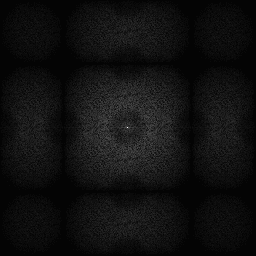
\includegraphics[width=\textwidth]{content/TemporalerAlg/Bilder/Sorting/Spektren/Ausschnitt4.png}
        \subcaption{FFT t=4}
        \label{pic:sorting_t4_FFT}
    \end{subfigure}
    \end{tcolorbox}
    \caption{Sorting ab t=1 aktiviert}
    \label{pic:Sorting_over_seven_frames}
\end{figure}


\begin{figure}[H]
    \centering 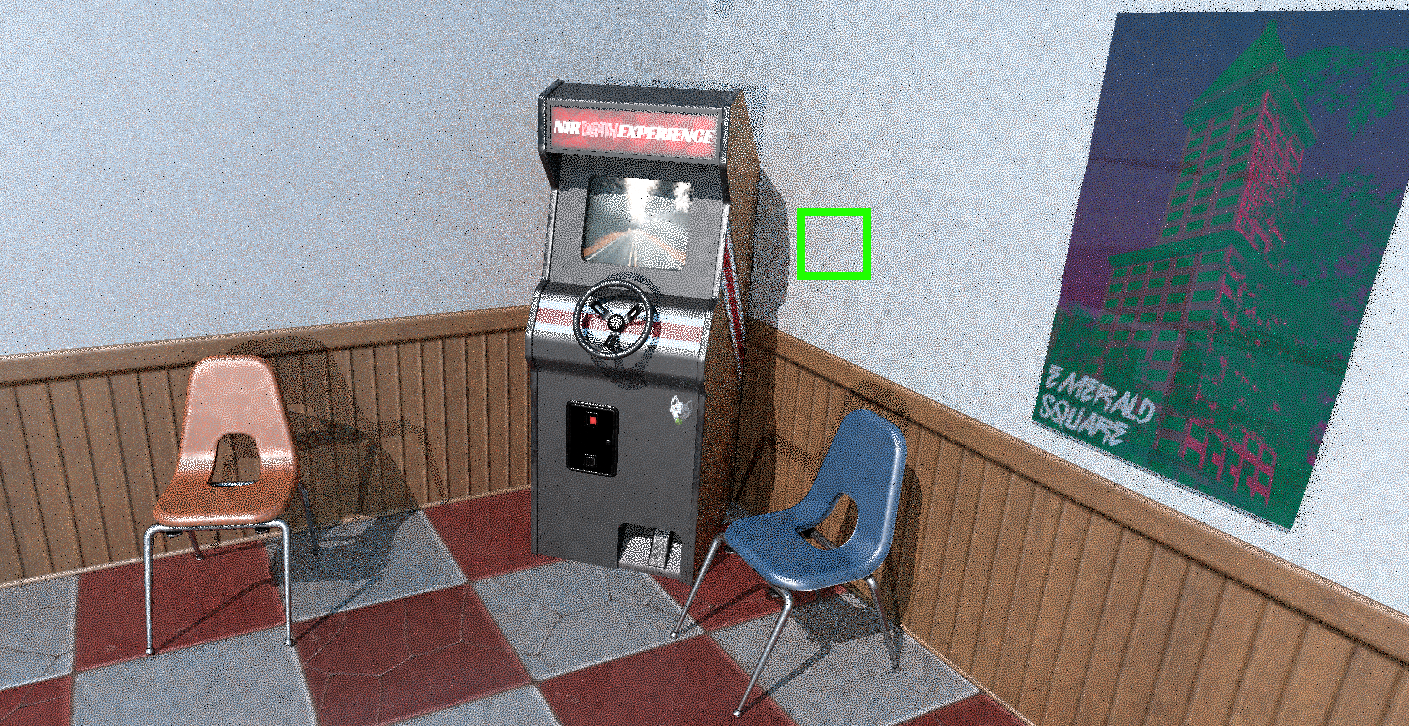
\includegraphics[scale=.25]{content/TemporalerAlg/Bilder/Sorting/Szene/Szene7.png}
    \caption{Szene}
    \label{fig:Nur_Sorting_Szene_t7}
\end{figure}

Die Bildreihe zeigt die ersten sieben erstellten Bilder mit ausschließlichem 
Sortieren(B=8) ohne \nameref{ch:Content2:sec:Retargeting}.

\begin{itemize}
    \item[t=1-2] Die ersten beiden erzeugten Bilder lassen keine blue noise Eigenschaften erkennen.
                    Das typische weiße Rauschen ist zu erkennen und hat einen unbefriedigenden optischen Eindruck.
                     \par 
                    
    \item[t=3] Ab dem dritten Bild können wir eine \nameref{ch:Content1:sec:blue noise} Eigenschaft im Bild durch ein 
                bloßes Sortieren erkennen. Die daraus resultierende Steigerung der optisch wahrnehmbaren 
                Qualität, wie bereits in Arbeiten wie \cite{3288} besprochen, lässt sich gut erkennen. 
    \item[t=4-7] Der blue noise Charakter kann auch über die darauffolgenden Bilder erhalten werden.
                Allerdings ist der Charakter noch nicht stark genug ausgeprägt. Hier lässt sich der zuvor beschriebene 
                Effekt erkennen: Durch die Benutzung einer neuen blue noise Textur in jedem Bild akkumulieren 
                Verbesserungen nicht so gut und das Spektrum hat einen mehr verschwommenen Charakter ohne hohen 
                Kontrast.
\end{itemize}

Diese Erkenntnisse veranlassen uns einen zusätzlichen Schritt nach dem Sortieren (vor der erneuten Bilderzeugung) 
einzuführen: Das \nameref{ch:Content2:sec:Retargeting}.